\chapter{\IfLanguageName{dutch}{Proof of concept}{State of the art}}%
\label{ch:proof-of-concept}

Dit deel van het onderzoek stelt een Proof of Concept voor die zich richt op het web scrapen van het netwerkverkeer van een website zodat de gestructureerde data die verstuurd wordt van de server kan onderschept worden. Sommige van deze bestanden die de server verstuurd, bevatten de gestructureerde data die de website gebruikt om zijn inhoud dynamisch te genereren. In deze gestructureerde data is vaak meer informatie te vinden dan op de website getoond wordt. Dit zorgt voor een verhoogde kwaliteit van verzamelde data. Het vergt ook minder rekenkracht van de machine dat de web scraper op uitgevoerd wordt omdat de HTML-code niet geparsed hoeft te worden. De Proof of Concept bestaat uit een Python script.

\section{Vereisten}
Het uitvoeren van deze Proof of Concept vereist bepaalde software op het systeem. De vereiste software zijn:
\begin{itemize}
    \item Python \footnote{\url{https://www.python.org/downloads/}}
    \item De package manager pip~\footnote{\url{https://pip.pypa.io/en/stable/installation/}}
\end{itemize}

\section{Versies}
In deze Proof of Concept wordt gebruik gemaakt van Python versie 3.10.2. De python-Bibliotheken die in deze Proof of Concept gebruikt zullen worden zijn:

\begin{itemize}
    \item \textbf{json: } Deze Python-bibliotheek wordt gebruikt om met JSON-bestanden te werken. json is standaard geinstalleerd in Python

    \item \textbf{Requests: } Deze Python-bibliotheek wordt gebruikt om HTTP-verzoeken te maken.

    \item \textbf{Selenium: } Selenium wordt gebruikt om het netwerkverkeer op te halen.
\end{itemize}

Om mogelijke conflicten tussen de gebruikte Python-bibliotheken te voorkomen wordt gebruik gemaakt van een virtuele Python omgeving. Om de virtuele omgeving te creëren moet het commando \ref{cmd:createvenv} uitgevoerd worden.

\begin{lstlisting}[language=bash, label={cmd:createvenv}, caption={Het commando om een virtuele Python omgeving te creëren}]
    python -m venv /path/to/new/virtual/environment/
\end{lstlisting}
Om de virtuele Python omgeving te activeren op een Windows machine moet het commando \ref{cmd:startvenv} uitgevoerd worden, voor een Linux of MacOS machine moet het commando \ref{bash:startvenv} gebruikt worden.
\begin{lstlisting}[language=bash, label={cmd:startvenv}, caption={Het commando om een virtuele Python omgeving te activeren op een Windows machine}]
    venv\Scripts\activate.bat
\end{lstlisting}

\begin{lstlisting}[language=bash, label={bash:startvenv}, caption={Het commando om een virtuele Python omgeving te activeren op een Linux of MacOS machine}]
    $ source myvenv/bin/activate
\end{lstlisting}

Om de gebruikte Python-bibliotheken te installeren moet het commando \ref{cmd:req.txt} uitgevoerd worden. het bestand \texttt{requirements.txt} is te vinden op de github-pagina \footnote{\url{https://github.com/hannesroegiers/bachelorproef/tree/main/PoC}}van deze Proof of Concept. Dit bestand bevat de nodige Python-bibliotheken met de gebruikte versie.
\begin{lstlisting}[language=bash, label={cmd:req.txt}, caption={Het commando om de nodige Python-bibliotheken te installeren}]
    pip install -r requirements.txt
\end{lstlisting}

\section{Verkenning}
Op de doel website\footnote{\url{https://www.oddsportal.com/football/belgium/jupiler-pro-league/}} zijn een aantal voetbal wedstrijden te zien. Naast iedere wedstrijd staan 3 kolommen zoals te zien in \ref{fig:website1}. De cijfers(betting odds voor de wedstrijden) die in deze kolommen staan zijn de data die de scraper gaat proberen te extraheren.

\begin{figure}[h]
    \centering
    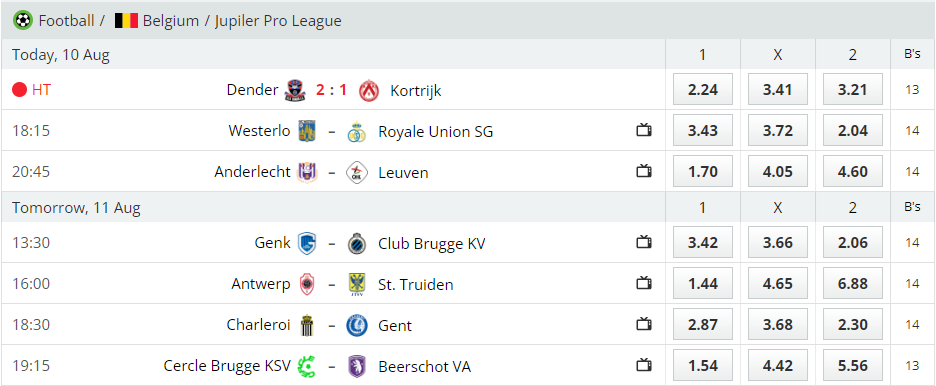
\includegraphics[width=\linewidth]{graphics/website1.png}
    \caption{De doel website}
    \label{fig:website1}
\end{figure}

\section{Analyse}
In deze tweede fase van het onderzoek wordt gebruikgemaakt van de Chrome-browser en de ingebouwde developer tools om het netwerkverkeer van een website te analyseren. De developer tools kunnen worden geopend door op de functietoets \texttt{F12} te drukken of door met de rechtermuisknop op een webpagina te klikken en vervolgens te kiezen voor \texttt{Inspect} of \texttt{Inspecteren}.
\\
Bij het laden van een website worden verschillende HTTP-verzoeken naar de server gestuurd, waarvan de antwoorden dienen om de inhoud van de website dynamisch op te bouwen. Deze HTTP-verzoeken en hun antwoorden zijn te vinden in het \texttt{Network}-tabblad van de developer tools, waar het netwerkverkeer van de website in detail wordt weergegeven.

Voor web scraping zijn twee specifieke tabbladen in de developer tools van beland: het \texttt{Elements}-tabblad en het \texttt{Network}-tabblad. In het \texttt{Elements}-tabblad kan de HTML-code en structuur van de website worden bekeken. Dit biedt inzicht in hoe de inhoud van de website is opgebouwd. In het \texttt{Network}-tabblad kan het netwerkverkeer tussen de client(de browser) en de server worden geanalyseerd, zoals geilustreerd in figuur~\ref{fig:networktab}.

\begin{figure}[h]
    \centering
    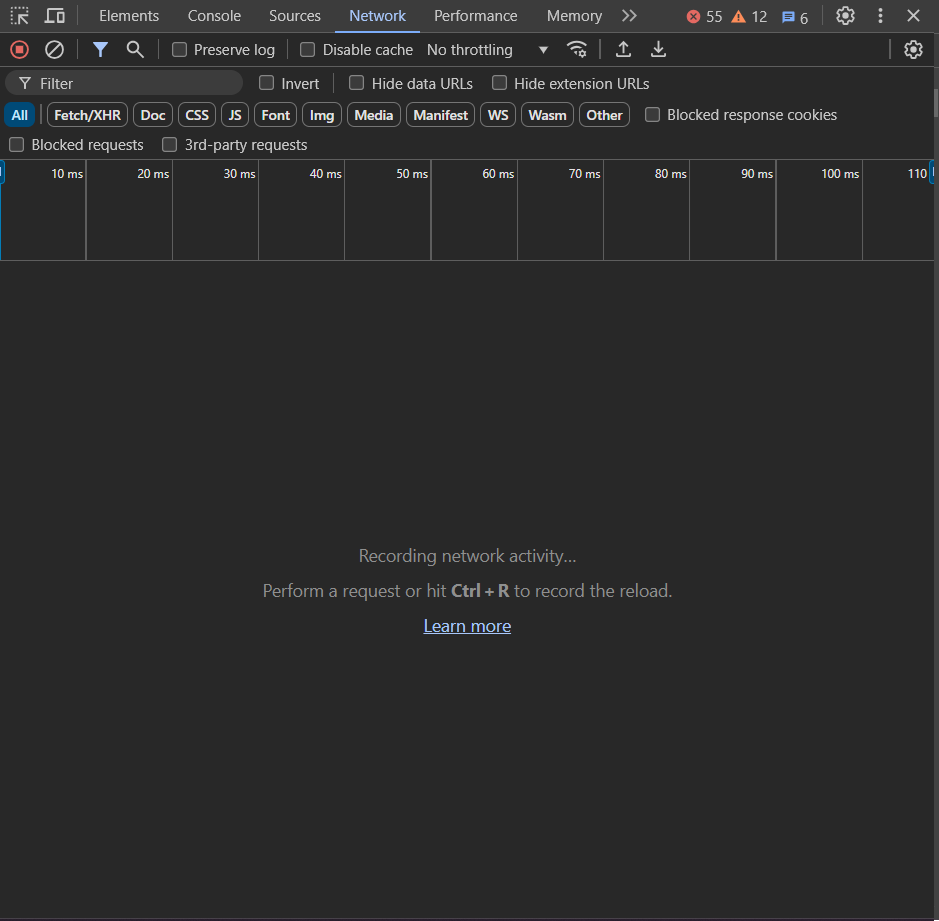
\includegraphics[width=\linewidth]{graphics/DevTools1.png}
    \caption{De developer tools, het netwerk tabblad}
    \label{fig:networktab}
\end{figure}

Wanneer de webpagina opnieuw wordt geladen, worden in het Network-tabblad alle netwerkverzoeken weergegeven die plaatsvinden tussen de client en de server, zoals te zien is in figuur~\ref{fig:networktab2}.

\begin{figure}[h]
    \centering
    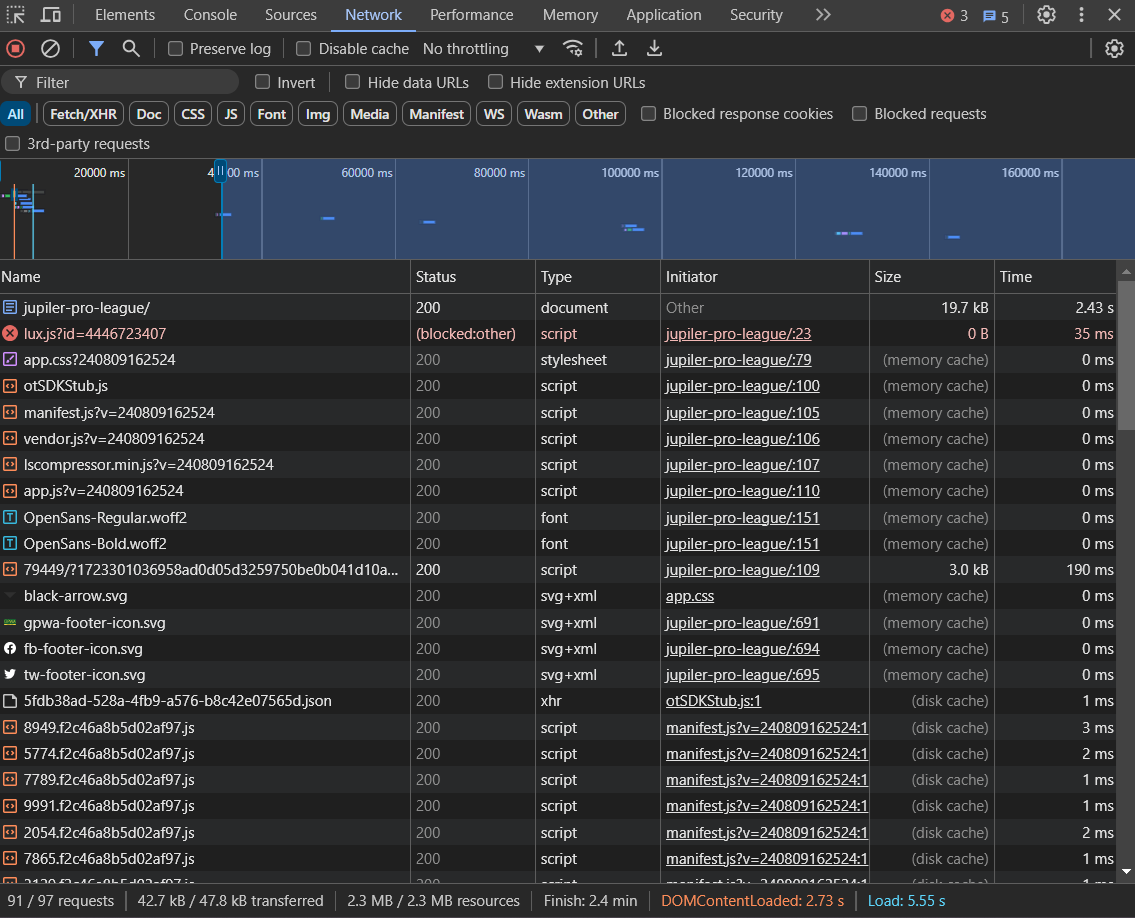
\includegraphics[width=\linewidth]{graphics/DevTools2.png}
    \caption{Het netwerkverkeer in de developer tools}
    \label{fig:networktab2}
\end{figure}

Hoewel er veel verschillende soorten bestanden worden uitgewisseld, richt dit onderzoek zich op bestanden die gestructureerde data bevatten. In de developer tools kan dit verkeer worden gefilterd door de optie \texttt{Fetch/XHR} te selecteren. Dit filter toont voornamelijk JSON- en XML-bestanden, die vaak belangrijke data bevatten voor verdere analyse.
Er blijven nu slechts 7 requests over~\ref{fig:networktab3}.

\begin{figure}[h]
    \centering
    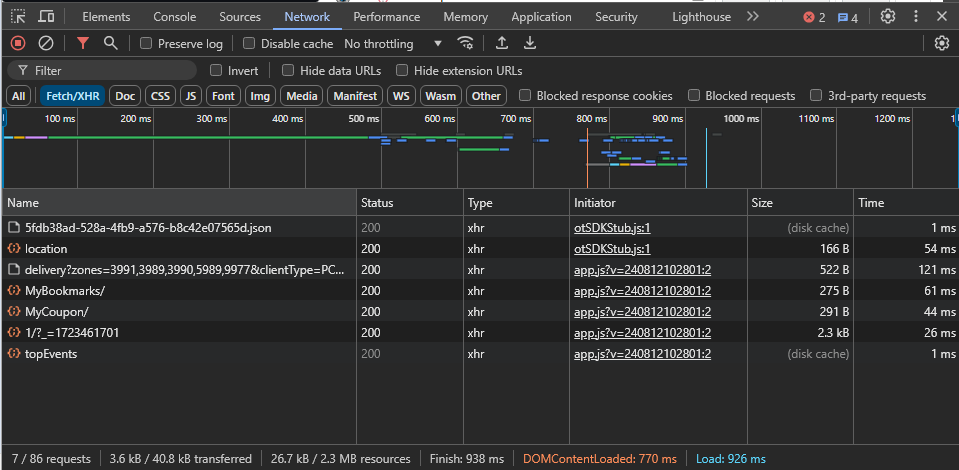
\includegraphics[width=\linewidth]{graphics/DevTools3.png}
    \caption{Het gefilterde netwerkverkeer in de developer tools}
    \label{fig:networktab3}
\end{figure}

De antwoorden van deze overblijvende HTTP-verzoeken bevatten allemaal JSON-bestanden. Na verdere analyse van deze bestanden is vast te stellen dat de betting odds terug te vinden zijn in het HTTP-verzoek dat een bestand met naam \texttt{?\_=1723461701} terug geeft.

\subsubsection{Bepalen van de web scraping methode}
De HTML-code van de doel website is complex, hierdoor is de code moeilijk te lezen en kleine veranderingen in de code kunnen ervoor zorgen de locatie van de betting odds verandert. De website wordt dynamisch opgebouwd met behulp van HTTP-verzoeken die gestructureerde data opvragen. Dit zorgt ervoor dat web scraping met netwerkverkeersanalyse bij deze website de beste keuze is.
\\
\\
In figuur~\ref{fig:networktab4} is te zien hoe de header van het HTTP-verzoek is opgebouwd. Indien de website een duidelijke en consistente structuur in de headers heeft, kan een Python-script worden ontwikkeld dat gebruik maakt van een loop om systematisch HTTP-requests te versturen. Deze aanpak maakt het mogelijk om alle benodigde data te verzamelen zonder de beperkingen van traditionele scraping-methoden die zich puur op de HTML-content richten.
\begin{figure}[h]
    \centering
    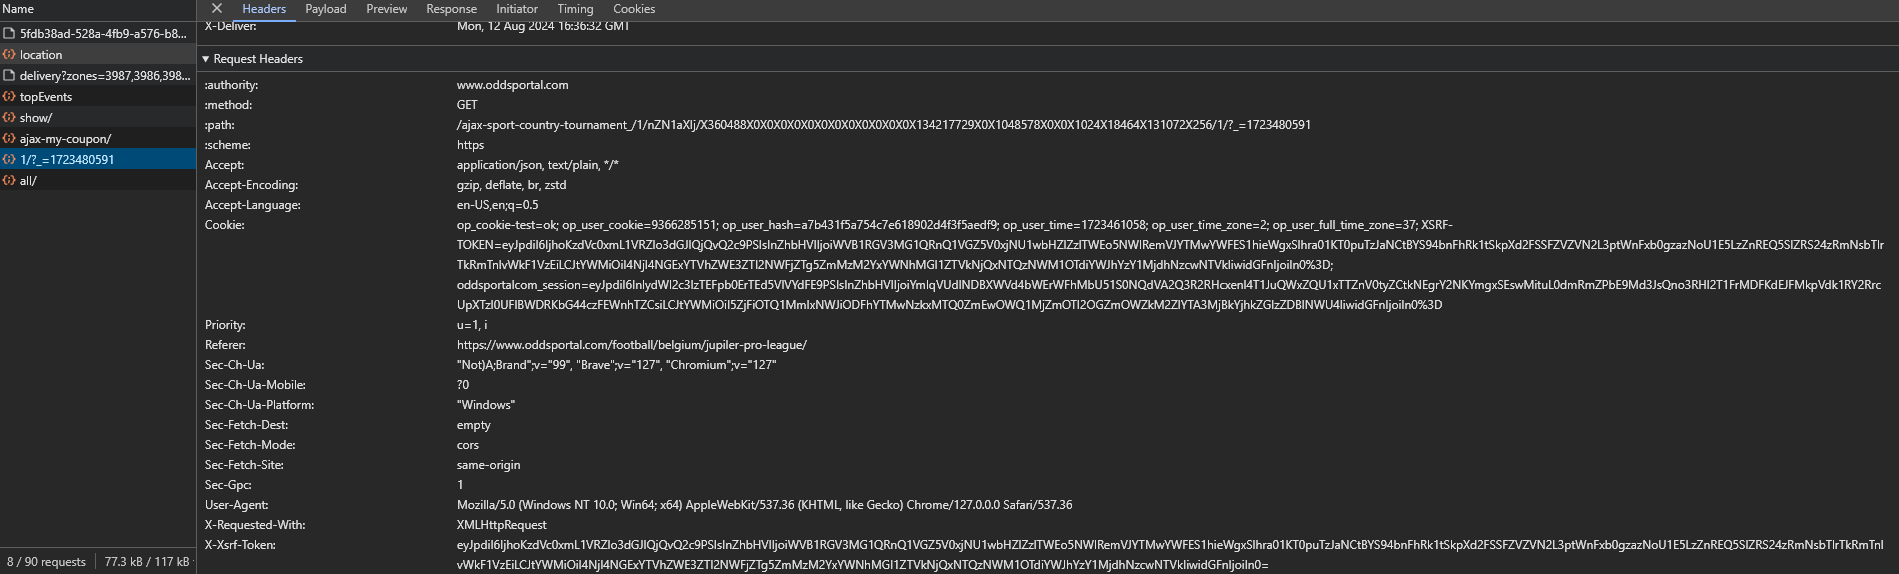
\includegraphics[width=\linewidth]{graphics/headers.png}
    \caption{De headers van het betting odds HTTP-verzoek}
    \label{fig:networktab4}
\end{figure}


De Python-loop stuurt hierbij een reeks gestructureerde HTTP-verzoeken naar de server van de doelwebsite. Door gebruik te maken van variabelen in de URL of parameters binnen de request headers, kan het script automatisch door verschillende datasets navigeren en deze extraheren. Dit minimaliseert de kans op blokkades door anti-scraping maatregelen en verhoogt de efficiëntie van de data-extractie. In code fragment~\ref{code:example5} is een voorbeeld te zien over web scrapen met netwerkverkeersanalyse wanneer de parameters in de HTTP-verzoek header gestructureerd en niet vertroebeld zijn.
\begin{listing}
    \begin{lstlisting}[language=python, captionpos=b, caption={Een voorbeeld van een eenvoudige webscraper.}, label={code:example5}]
        import requests

        # Dummy URL: https://www.oddsportal.com/ajax-sport-country-tournament/sport/country/league/

        # Deze arrays kunnen manueel onderhouden worden of opgehaald worden met een API
        request_parameters = {
            "Voetbal": {
                "Belgie": ["Jupiler Pro League", "Eerste klasse B"],
                "Nederland": ["Eredivisie", "Eerste Divisie"],
                "Engeland": ["Premier League", "Championship"],
            },
            "Hockey": {
                "België": ["Belfius Hockey League"],
                "Nederland": ["Hoofdklasse", "Promotieklasse"],
                "Duitsland": ["Bundesliga"],
            },
            "Tennis": {
                "Internationaal": ["ATP Tour", "WTA Tour"],
                "Verenigde Staten": ["US Open Series"],
                "Australie": ["Australian Open"],
            }
        }

        # Overlopen van alle url parameters
        for sport, countries in request_parameters.items():
            for country, leagues in countries.items():
                for league in leagues:
                    request_string = f"https://www.oddsportal.com/ajax-sport-country-tournament/{sport}/{country}/{league}/"

                    r = requests.get(request_string)
    \end{lstlisting}
\end{listing}

Na een grondige analyse van het HTTP-verzoek kan worden geconcludeerd dat er geen duidelijke en consistente structuur aanwezig is in het verzoek. De parameters die in het verzoek worden gebruikt, lijken opzettelijk vertroebeld (geobfusceerd) te zijn, waardoor ze bestaan uit willekeurige tekens zonder directe betekenis. Dit maakt het onmogelijk om de inhoud en betekenis van deze parameters zonder meer te interpreteren. Om enige nuttige informatie hieruit te kunnen destilleren, zou het noodzakelijk zijn om de bijbehorende JavaScript-code te reverse-engineeren. Dit proces zou echter aanzienlijke tijd en diepgaande technische kennis vereisen.
\\ \\
Een van de parameters in het verzoek komt overeen met het bestand dat als antwoord wordt teruggestuurd. Hoewel de inhoud van dit bestand constant blijft bij het herladen van de pagina, verandert de naam van het bestand bij elke herlaadbeurt, het enige dat consistent blijft bij deze naam is dat het start met \texttt{?\_=17}. Deze naamwijziging voegt een extra laag van complexiteit toe, waardoor verdere analyse van deze parameter bijzonder uitdagend is.
\\ \\
De web scraping methode die zal worden toegepast voor deze website maakt gebruik van netwerkverkeersanalyse. Het volledige netwerkverkeer zal worden opgehaald en dan daarna gefilterd worden op bestandstype, naam en inhoud. De focus zal liggen op robuustheid en minimaal onderhoud.

